%Version 3.1 December 2024
% See section 11 of the User Manual for version history
%
%%%%%%%%%%%%%%%%%%%%%%%%%%%%%%%%%%%%%%%%%%%%%%%%%%%%%%%%%%%%%%%%%%%%%%
%%                                                                 %%
%% Please do not use \input{...} to include other tex files.       %%
%% Submit your LaTeX manuscript as one .tex document.              %%
%%                                                                 %%
%% All additional figures and files should be attached             %%
%% separately and not embedded in the \TeX\ document itself.       %%
%%                                                                 %%
%%%%%%%%%%%%%%%%%%%%%%%%%%%%%%%%%%%%%%%%%%%%%%%%%%%%%%%%%%%%%%%%%%%%%

%%\documentclass[referee,sn-basic]{sn-jnl}% referee option is meant for double line spacing

%%=======================================================%%
%% to print line numbers in the margin use lineno option %%
%%=======================================================%%

%%\documentclass[lineno,pdflatex,sn-basic]{sn-jnl}% Basic Springer Nature Reference Style/Chemistry Reference Style

%%=========================================================================================%%
%% the documentclass is set to pdflatex as default. You can delete it if not appropriate.  %%
%%=========================================================================================%%

%%\documentclass[sn-basic]{sn-jnl}% Basic Springer Nature Reference Style/Chemistry Reference Style

%%Note: the following reference styles support Namedate and Numbered referencing. By default the style follows the most common style. To switch between the options you can add or remove “Numbered” in the optional parenthesis. 
%%The option is available for: sn-basic.bst, sn-chicago.bst%  
 
%%\documentclass[pdflatex,sn-nature]{sn-jnl}% Style for submissions to Nature Portfolio journals
%%\documentclass[pdflatex,sn-basic]{sn-jnl}% Basic Springer Nature Reference Style/Chemistry Reference Style
\documentclass[pdflatex,sn-mathphys-num]{sn-jnl}% Math and Physical Sciences Numbered Reference Style
%%\documentclass[pdflatex,sn-mathphys-ay]{sn-jnl}% Math and Physical Sciences Author Year Reference Style
%%\documentclass[pdflatex,sn-aps]{sn-jnl}% American Physical Society (APS) Reference Style
%%\documentclass[pdflatex,sn-vancouver-num]{sn-jnl}% Vancouver Numbered Reference Style
%%\documentclass[pdflatex,sn-vancouver-ay]{sn-jnl}% Vancouver Author Year Reference Style
%%\documentclass[pdflatex,sn-apa]{sn-jnl}% APA Reference Style
%%\documentclass[pdflatex,sn-chicago]{sn-jnl}% Chicago-based Humanities Reference Style

%%%% Standard Packages
%%<additional latex packages if required can be included here>

\usepackage{graphicx}%
\usepackage{multirow}%
\usepackage{amsmath,amssymb,amsfonts}%
\usepackage{amsthm}%
\usepackage{mathrsfs}%
\usepackage[title]{appendix}%
\usepackage{xcolor}%
\usepackage{textcomp}%
\usepackage{manyfoot}%
\usepackage{booktabs}%
\usepackage{algorithm}%
\usepackage{algorithmicx}%
\usepackage{algpseudocode}%
\usepackage{listings}%
\setlength{\parindent}{0pt}
\usepackage[utf8]{inputenc}
\usepackage[T1]{fontenc}
\hypersetup{colorlinks=true, linkcolor=black, citecolor=black, urlcolor=black}
%%%%

%%%%%=============================================================================%%%%
%%%%  Remarks: This template is provided to aid authors with the preparation
%%%%  of original research articles intended for submission to journals published 
%%%%  by Springer Nature. The guidance has been prepared in partnership with 
%%%%  production teams to conform to Springer Nature technical requirements. 
%%%%  Editorial and presentation requirements differ among journal portfolios and 
%%%%  research disciplines. You may find sections in this template are irrelevant 
%%%%  to your work and are empowered to omit any such section if allowed by the 
%%%%  journal you intend to submit to. The submission guidelines and policies 
%%%%  of the journal take precedence. A detailed User Manual is available in the 
%%%%  template package for technical guidance.
%%%%%=============================================================================%%%%

%% as per the requirement new theorem styles can be included as shown below
\theoremstyle{thmstyleone}%
\newtheorem{theorem}{Theorem}%  meant for continuous numbers
%%\newtheorem{theorem}{Theorem}[section]% meant for sectionwise numbers
%% optional argument [theorem] produces theorem numbering sequence instead of independent numbers for Proposition
\newtheorem{proposition}[theorem]{Proposition}% 
%%\newtheorem{proposition}{Proposition}% to get separate numbers for theorem and proposition etc.

\theoremstyle{thmstyletwo}%
\newtheorem{example}{Example}%
\newtheorem{remark}{Remark}%

\theoremstyle{thmstylethree}%
\newtheorem{definition}{Definition}%

\raggedbottom
%%\unnumbered% uncomment this for unnumbered level heads

\begin{document}

\title[Article Title]{Domain shift in distilled T5-based models for language translation tasks}

%%=============================================================%%
%% GivenName	-> \fnm{Joergen W.}
%% Particle	-> \spfx{van der} -> surname prefix
%% FamilyName	-> \sur{Ploeg}
%% Suffix	-> \sfx{IV}
%% \author*[1,2]{\fnm{Joergen W.} \spfx{van der} \sur{Ploeg} 
%%  \sfx{IV}}\email{iauthor@gmail.com}
%%=============================================================%%

\author{\fnm{Giovanni} \sur{Novati}}

\affil{\orgdiv{Computer Science Master's Course}, \orgname{Universit\'a degli Studi di Milano}}

%%==================================%%
%% Sample for unstructured abstract %%
%%==================================%%

\abstract{In this work we investigate about black-box knowledge distillation from a GPT-5 Mini teacher for language translation tasks, by training four student models from the T5-Efficient and mT5 architectures on two different domains. Using only the predictions generated by the teacher, we evaluate in-domain and out-of-domain predictions, using chrF++ and BLEU metrics. Results show that models with more parameters have stronger translation and generalization quality, multilingual pretraining provides a significant advantage, and with mixed domain training you can mitigate domain shift by paying a small cost in overall performance.}

%%================================%%
%% Sample for structured abstract %%
%%================================%%

% \abstract{\textbf{Purpose:} The abstract serves both as a general introduction to the topic and as a brief, non-technical summary of the main results and their implications. The abstract must not include subheadings (unless expressly permitted in the journal's Instructions to Authors), equations or citations. As a guide the abstract should not exceed 200 words. Most journals do not set a hard limit however authors are advised to check the author instructions for the journal they are submitting to.
	
\keywords{distillation, domain shift, language translation, t5, mt5}

\maketitle
\setlength{\parskip}{1em}

\section{Introduction}\label{sec1}

In recent years, more and more cumbersome LLMs have come to life in the AI race led by OpenAI and joined by all other competitors and big techs like Google, Anthropic, and Meta, just to say some. These companies have created models with billions if not trillions of parameters \cite{abacha2025medec}, and are general purpose, which means they are capable of doing a wide range or tasks such as natural language understanding and generation, decision making, and reasoning \cite{ye2025llms4allreviewlargelanguage}.

The main downside of these models is also their main advantage: the size. Running inference requires expensive hardware in order to load all parameters into dedicated GPU memory. Moreover, if we want to perform a task that only uses a subset of the model capabilities, all the parameters are still active, leading to a waste of memory and computational power.

In the case we only want to perform a certain task, it might be useful to condense a larger model into a smaller one, specialized on that specific task while preserving comparable performance. This process is commonly known ad distillation \cite{hinton2015distilling}, and consists in transferring knowledge from a teacher model into a smaller student model.

A limitation arises when the teacher model we want to use is proprietary, and internal parameters or output logits are not accessible. Using a black-box makes the distillation process more difficult, and in those scenarios alternative strategies must be considered. One of them is training the student using only teacher's predictions; in this way we are still able to train the smaller model, but a reduction in performance is expected compared to full logits distillation \cite{yang2025survey}.

In this paper, we investigate the distillation of task-specific student models from a GPT-5 Mini teacher using only its output predictions. We test two different student architectures across multiple parameter counts in order to assess their performance under domain shift. The models are trained on English-to-Italian translation and evaluated using BLEU and chrF++ metrics to measure both in-domain and out-of-domain effectiveness. Many more metrics like COMET and TER exists, but in order to keep thinks simple I decided to focus only on those two.

\section{Methodology}\label{sec2}

\subsection{Task}\label{sec2.1}

First, let's define the task of interest. I wanted to train the model on something useful and challenging, in order to stress the student and understand its limitations. I opted for a translation task, specifically English to Italian, since translating into morphologically richer languages is a more difficult task \cite{chahuneau2013translating} compared to the opposite. Italian is a more complex language as it has more verb tenses, and information like gender and number is embedded into words. These elements are not always present into English sentences and must be inferred based on the context.

\subsection{Datasets}\label{sec2.2}

Two domains were defined to train and evaluate the students.. Dataset $A$ \cite{charles_kelly_2020} contains 175.622 couples of English sentences with their related French translation. These sentences cover everyday life situations, with an average length of 42 characters. The second one, Dataset $B$ \cite{agentlans2023highquality}, contains 1.534.699 english sentences with an average length of 133 characters, and are related to educational and academic contexts. Note that the author of the latter one says that the dataset may introduce some biases, like a more formal writing style. Table~\ref{tab:dataset_examples} shows examples from both datasets.

\begin{table}[h]
	\centering
	\renewcommand{\arraystretch}{1.5}
	\begin{tabular}{p{0.15\textwidth} p{0.75\textwidth}}
		\hline
		\textbf{Source} & \textbf{Example sentences} \\
		\hline
		Dataset A	& I'll get something to drink for both of you. \\
					& I have to do my best. \\
					& I'm going to wear these shoes on our date tonight. \\
		\hline
		Dataset B	& Muscles, tendons, and ligaments depend upon proper joint movement to function at optimal levels. \\
					& It is advisable to keep water levels some distance below where the tiles are to prevent any damage. \\
					& Technological development has also contributed to long-term efficiency and productivity. \\
		\hline
	\end{tabular}
	\caption{Comparison of sample sentences from Dataset A and Dataset B.}
	\label{tab:dataset_examples}
\end{table}

Then, 35.000 sentences were extracted for training, 5.000 for validation and another 5.000 for testing from each dataset \cite{vieira2024much}, and final datasets were created to be used in the experiments. Since Dataset A consists of English-French pairs, the French side was discarded and only the English sentences were kept.

Next, using OpenAI API, GPT-5 Mini all English sentences were translated into Italian, and the resulting source-target pairs were saved in a CSV file. After completing the translations, an equal number of samples were extracted from Dataset A and Dataset B, and merged into a new Dataset AB, which combined the two domains. GPT-5 Mini was chosen in order to keep costs low; using a more advanced model such as GPT-5.2 would have increased the total cost by approximately 10 times.

Since GPT-5 Mini translations are used as reference labels, the evaluation metrics measure how closely a student has replicated the teacher's output. A perfect student would have a chrF++ of 100 against the teacher translation; that does not mean that the translation is perfect in an absolute way, but that student can perfectly imitate the teacher.

\subsection{Models}\label{sec2.3}

The model architectures decided to be used as students come from Google T5-Efficient and mT5 families \cite{tay2021scale}. These models come with different parameter count, and are pretrained with the Colossal, Cleaned Common Crawl Dataset \cite{commoncrawl}. The T5 family model and tokenizer are pretrained using only English sentences, while mT5 models are multilingual and support 101 different languages, Italian included.

For this study, both T5 and mT5 variants were tested in order to investigate wether a multilingual model have advantages on cross-lingual knowledge distillation, or if monolingual models with proper finetuning can also achieve similar performance on Italian translation tasks.

In particular, the models used for these experiments are T5-Efficient-Small, T5-Efficient-Base, mT5-Small, and mT5-Base. The parameter count of each model is shown in Table~\ref{tab:parameter_count}.

\begin{table}[h]
	\centering
	\renewcommand{\arraystretch}{1.5}
	\begin{tabular}{p{0.30\textwidth} p{0.20\textwidth}}
		\hline
		\textbf{Name} & \textbf{Parameter } \\
		\hline
		T5-Efficient-Small & 60M \\
		T5-Efficient-Base & 220M \\
		mT5-Small & 300M \\
		mT5-Base & 580M \\
		\hline
	\end{tabular}
	\caption{Parameter count of the models used.}
	\label{tab:parameter_count}
\end{table}

\subsection{Training}\label{sec2.4}

Each model listed in Table~\ref{tab:parameter_count} was fine-tuned on the three different datasets resulting in three variants per base model: Student A, Student B, and Student AB.

In total, 12 models were fine-tuned for 30 epochs on a machine provided by the MIPS Laboratory, equipped with an NVIDIA 3090 (24GB), an Intel i9-12900K, and 64GB of system RAM. All models were trained using 16 bits floating point, batches of size 16, a learning rate of 2e-5, and chrF++ as metric for evaluating the best model. For a more specific hyperparameter configuration, see code in \texttt{train\_student.py}. The training of all 12 models took about two days. 

\section{Results}\label{sec3}

Figure~\ref{fig:losses} shows the training and validation loss curves for all 12 models. All fine-tuned models converged within approximately 10 epochs, which was influenced by both model architecture and dataset characteristics. Multilingual models with higher parameter counts (mT5-Small and mT5-Base) converged faster than their monolingual counterparts (T5-Efficient-Small and T5-Efficient-Base). This effect was more pronounced on Dataset B, which contains longer sentences, more technical vocabulary, and greater context-dependency compared to Dataset A, which consists of shorter sentences with simpler vocabulary.

\begin{figure}[htbp]
	\centering
	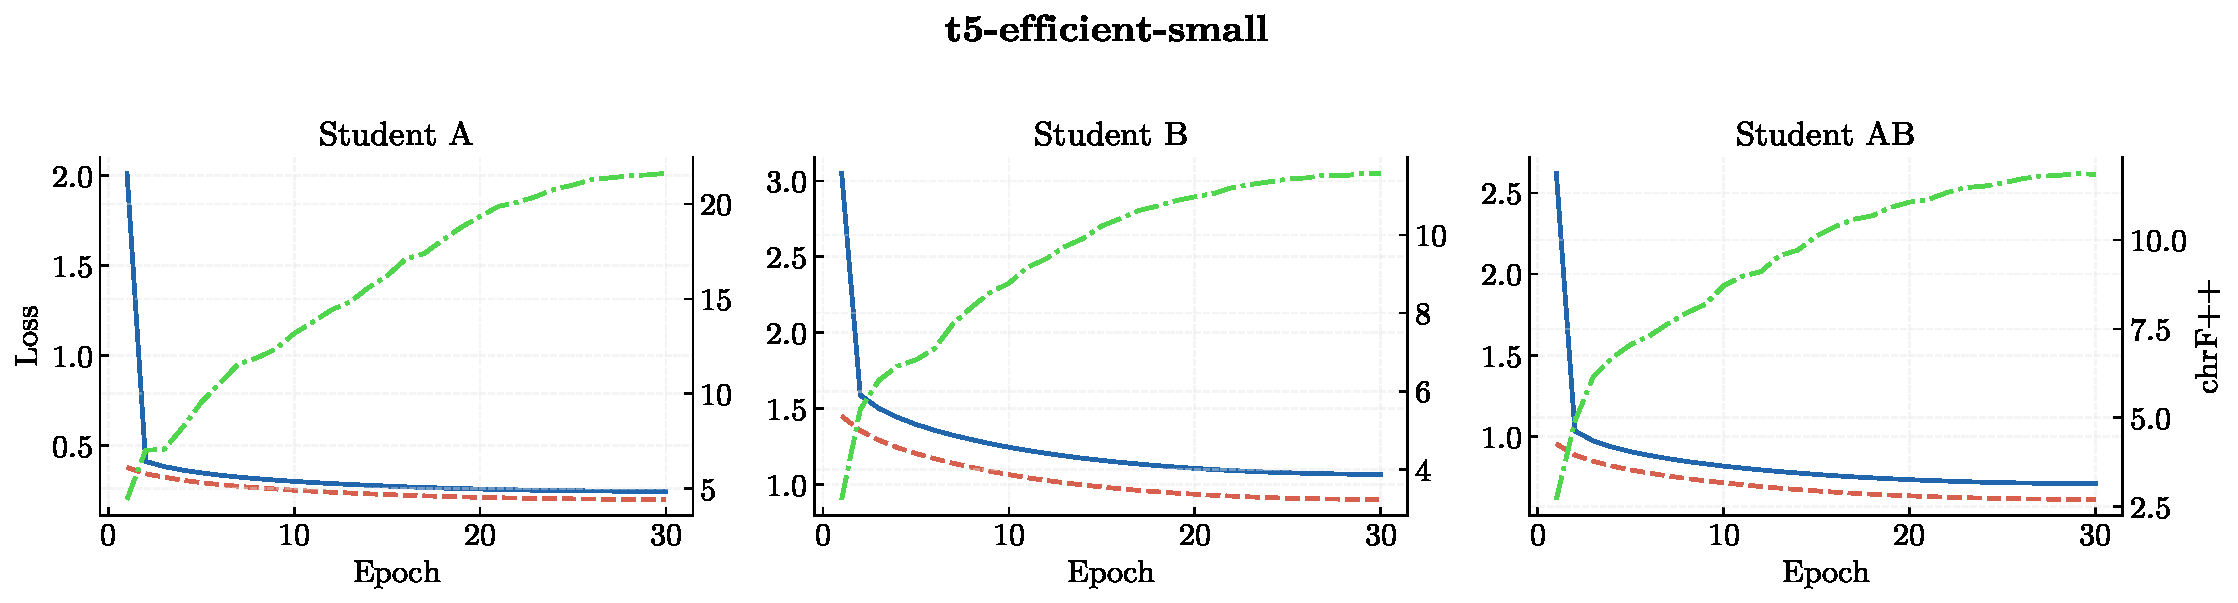
\includegraphics[width=\textwidth]{images/t5-efficient-small_losses.pdf}
	\centering
	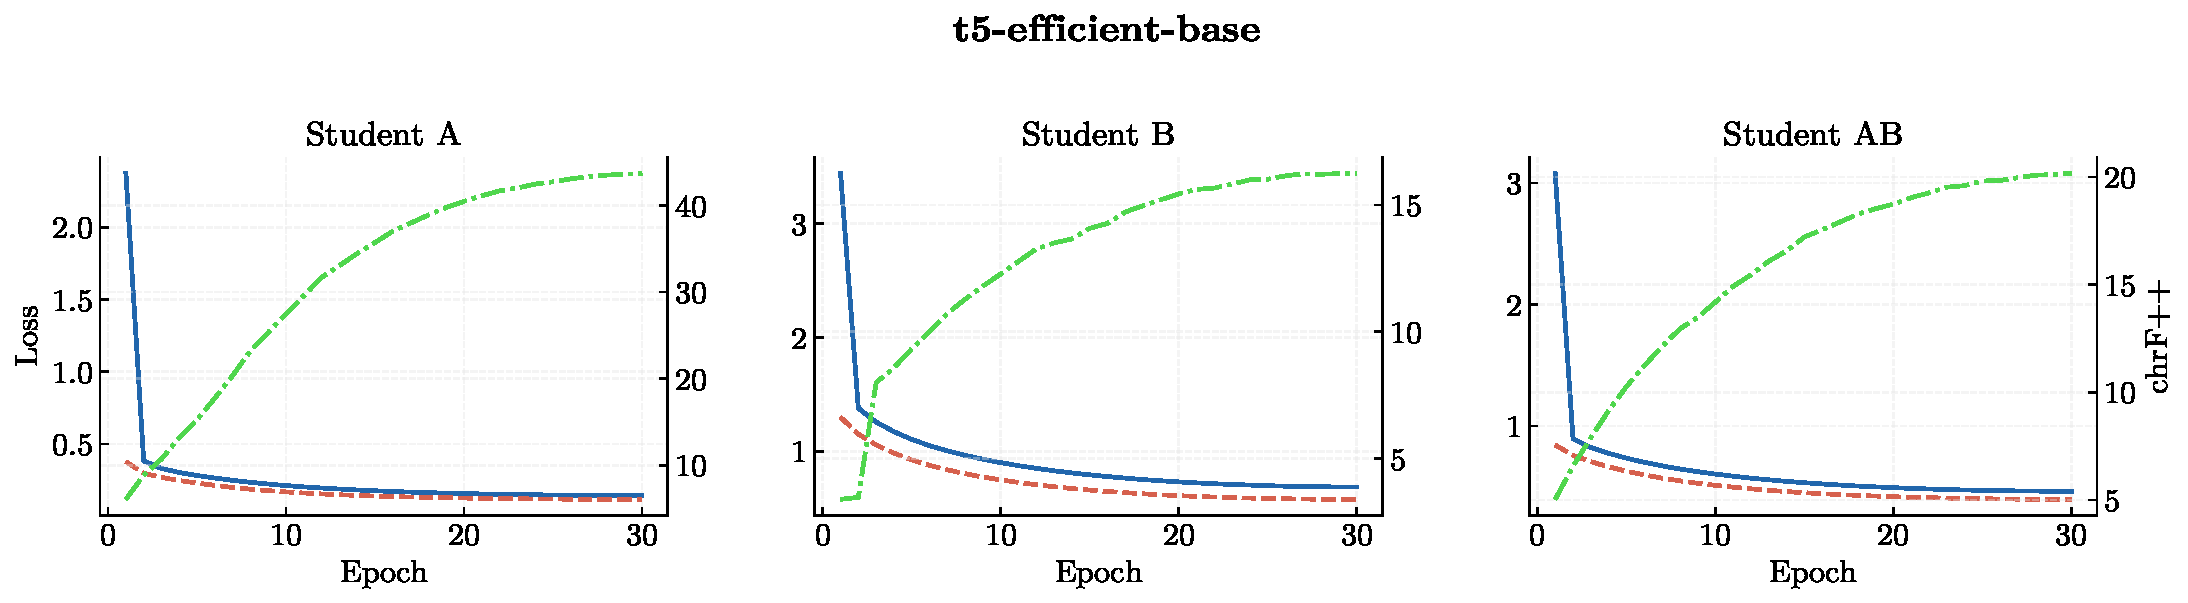
\includegraphics[width=\textwidth]{images/t5-efficient-base_losses.pdf}
	\centering
	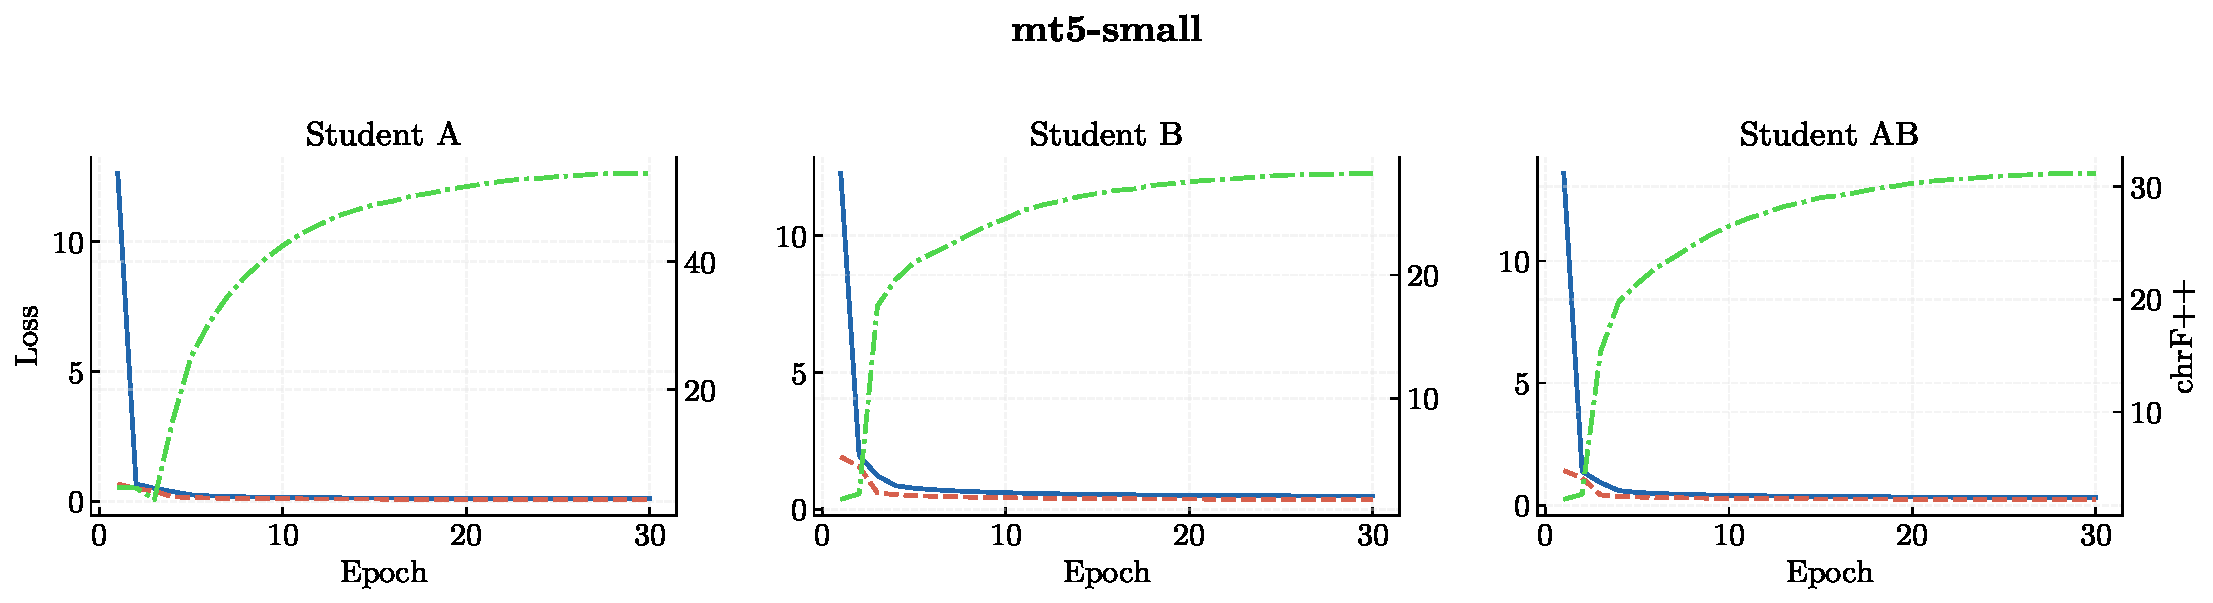
\includegraphics[width=\textwidth]{images/mt5-small_losses.pdf}
	\centering
	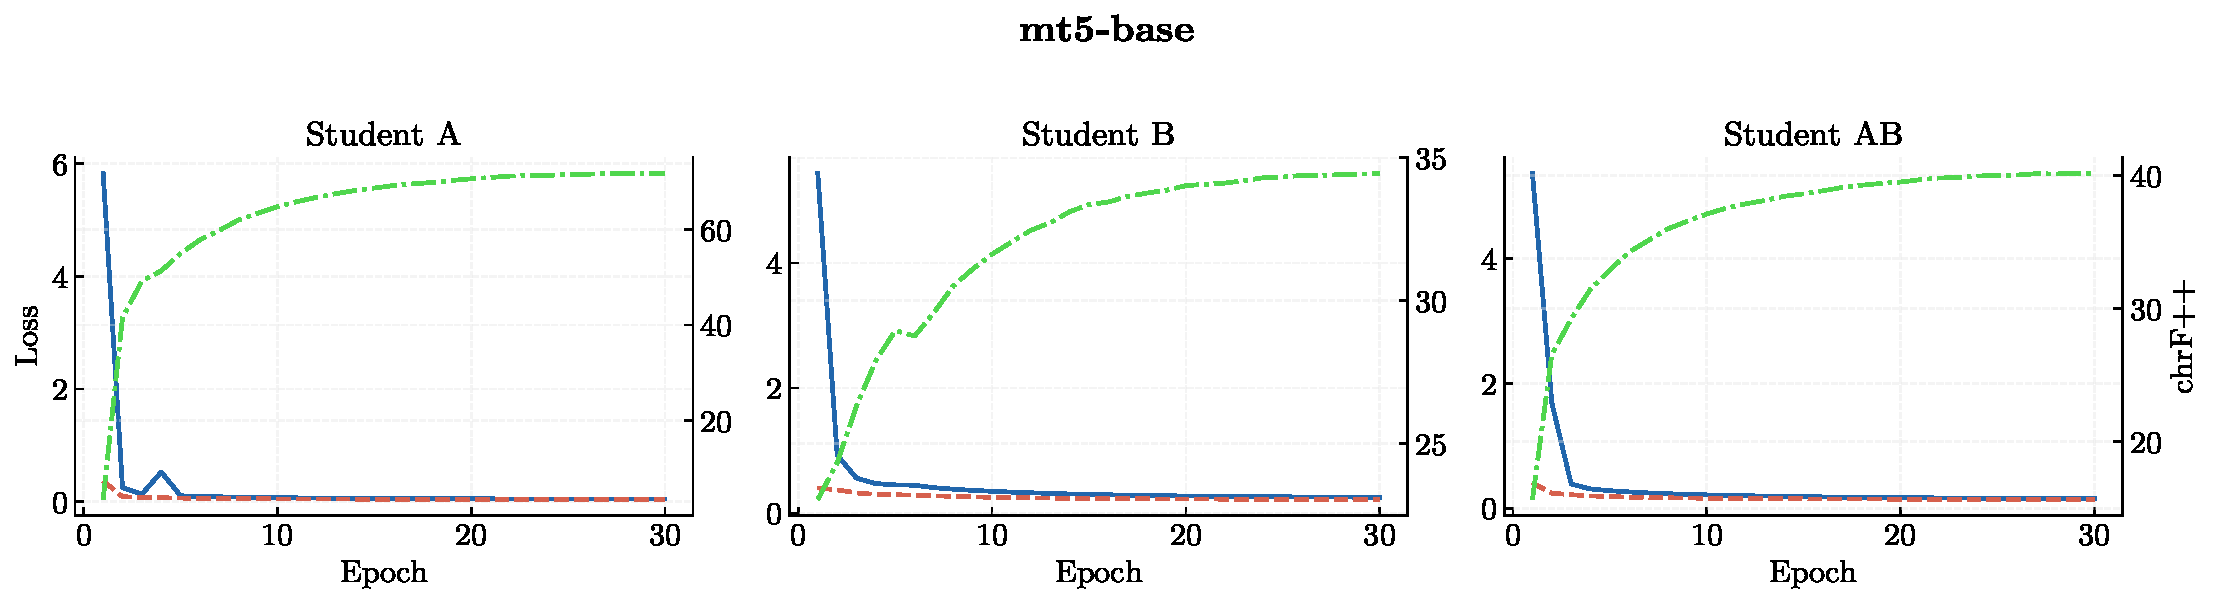
\includegraphics[width=\textwidth]{images/mt5-base_losses.pdf}
	\caption{Training loss (blue line), evaluation loss (orange line), and chrF++ metric (green line) for all models.}
	\label{fig:losses}
\end{figure}

\subsection{In-domain performance}

The chrF++ scores computed on validation data (Figure~\ref{fig:losses}) demonstrate that model size positively correlates with in-domain performance across all datasets. mT5-Base consistently achieves the highest scores, while T5-Efficient-Small shows the lowest performance. This behavior holds for both domain specific models (Student A and Student B) and the mixed domain model (Student AB).

\subsection{Out-of-domain generalization}

All scores are computed using GPT-5 Mini translations as reference, and measure how well a student can replicate the teacher. In this case the teacher represents the maximum performance achievable, and the gap between 100 and the student scores quantifies the cost of compression.

Table~\ref{tab:main_results} presents both in-domain and out-of-domain performance for all models using chrF++ and BLEU metrics. Bold values indicate the in-domain performance.

\begin{table}[htbp]
	\centering
	\renewcommand{\arraystretch}{1.3}
	\begin{tabular}{lccccc}
		\hline
		\multirow{2}{*}{\textbf{Model}} & \multirow{2}{*}{\textbf{Domain}} & \multicolumn{2}{c}{\textbf{chrF++}} & \multicolumn{2}{c}{\textbf{BLEU}} \\
		\cmidrule(lr){3-4} \cmidrule(lr){5-6}
		&  & \textbf{A} & \textbf{B} & \textbf{A} & \textbf{B} \\
		\hline
		T5-Efficient-Small & A & \textbf{22.1} & 10.6 & \textbf{4.1} & 0.4 \\
		T5-Efficient-Small & B & 17.2 & \textbf{24.6} & 2 & \textbf{5.2} \\
		T5-Efficient-Small & AB & \textbf{18.2} & \textbf{20.1} & \textbf{2.4} & \textbf{3.3} \\
		\hline
		T5-Efficient-Base & A & \textbf{45.1} & 19 & \textbf{23.2} & 1.7 \\
		T5-Efficient-Base & B & 26 & \textbf{41.4} & 6.1 & \textbf{15.4} \\
		T5-Efficient-Base & AB & \textbf{38.1} & \textbf{37.8} & \textbf{16} & \textbf{12.7} \\
		\hline
		mT5-Small & A & \textbf{53.6} & 29.8 & \textbf{33.2} & 6.5 \\
		mT5-Small & B & 39.7 & \textbf{52.6} & 16.8 & \textbf{25.9} \\
		mT5-Small & AB & \textbf{49} & \textbf{49.4} & \textbf{27.6} & \textbf{22.4} \\
		\hline
		mT5-Base & A & \textbf{71.1} & 45.9 & \textbf{56} & 19.1 \\
		mT5-Base & B & 54.3 & \textbf{65.3} & 32.8 & \textbf{42.5} \\
		mT5-Base & AB & \textbf{66.5} & \textbf{64.2} & \textbf{49.2} & \textbf{40.8} \\
		\hline
	\end{tabular}
	\vspace{4pt}
	\caption{In-domain and out-of-domain performance for all models evaluated with chrF++ and BLEU.}
	\label{tab:main_results}
\end{table}

Models fine-tuned on a single domain exhibit substantial performance degradation when evaluated on the other domain. For example, mT5-Base trained on Domain A achieves a chrF++ score of 71.1 on Domain A but only 45.9 on Domain B. This domain shift effect is consistent across all model architectures, with smaller models showing more severe degradation.

The Student AB models, trained on the combined dataset, achieve more balanced performance across both domains. While these models do not match the peak in-domain scores of domain-specific models, they demonstrate superior generalization. For instance, mT5-Base trained on Domain AB achieves chrF++ scores of 66.5 and 64.2 on Domains A and B respectively, compared to 71.1 and 45.9 for the domain specific mT5-Base model trained on Domain A.

In Table~\ref{tab:translation_examples} are also reported example of translations of two sentences: one coming from Dataset A and one from Dataset B. The chosen English sentence from Dataset A is \textit{"I've heard that some people sleep in bathtubes."}, while the one from Dataset B is \textit{"In 2003, for example, the murder rate in the 12 states without the death penalty was 4.1 for every 100,000 people."}.

\begin{table}[htbp]
	\centering
	\renewcommand{\arraystretch}{1.3}
	\begin{tabular}{p{0.2\linewidth} c p{0.4\linewidth} p{0.4\linewidth}}
		\hline
		\textbf{Model} & \textbf{Domain} & \textbf{Translation A} & \textbf{Translation B} \\
		\hline
		GPT-5 Mini & & Ho sentito che alcune persone dormono nelle vasche da bagno. & Nel 2003, ad esempio, il tasso di omicidi nei 12 stati senza pena di morte era di 4,1 ogni 100.000 persone. \\
		T5-Efficient-Small & A & Ho savo che persone sarebbe a scuola in settimana. & In 2003, il tuo è stato a scuola è stato a scuola a scuola è stato a scuola a scuola è stato a tutti i miei sul tuo giorno a scuola è stato a tutti i giorni a scuola è è stato è stato è stato è stato è stato è stato è stato è stato è stato è stato è stato è stato è stato è stato è stato è stato è stato è stato è stato \\
		T5-Efficient-Small & B & Ho sentito che alcune persone dormono nelle vasche da bagno. & Nel 2003, ad esempio, il tasso di omicidi nei 12 stati senza pena di morte era di 4,1 ogni 100.000 persone. \\
		T5-Efficient-Small & AB & Ho sentito che alcune persone dormono nelle vasche da bagno. & Nel 2003, ad esempio, il tasso di omicidi nei 12 stati senza pena di morte era di 4,1 ogni 100.000 persone. \\
		T5-Efficient-Base & A & Ho sentito che alcune persone dormono nelle vasche da bagno. & Nel 2003, ad esempio, il tasso di omicidi nei 12 stati senza pena di morte era di 4,1 ogni 100.000 persone. \\
		T5-Efficient-Base & B & Ho sentito che alcune persone dormono nelle vasche da bagno. & Nel 2003, ad esempio, il tasso di omicidi nei 12 stati senza pena di morte era di 4,1 ogni 100.000 persone. \\
		T5-Efficient-Base & AB & Ho sentito che alcune persone dormono nelle vasche da bagno. & Nel 2003, ad esempio, il tasso di omicidi nei 12 stati senza pena di morte era di 4,1 ogni 100.000 persone. \\
		mT5-Small & A & Ho sentito che alcune persone dormono nelle vasche da bagno. & Nel 2003, ad esempio, il tasso di omicidi nei 12 stati senza pena di morte era di 4,1 ogni 100.000 persone. \\
		mT5-Small & B & Ho sentito che alcune persone dormono nelle vasche da bagno. & Nel 2003, ad esempio, il tasso di omicidi nei 12 stati senza pena di morte era di 4,1 ogni 100.000 persone. \\
		mT5-Small & AB & Ho sentito che alcune persone dormono nelle vasche da bagno. & Nel 2003, ad esempio, il tasso di omicidi nei 12 stati senza pena di morte era di 4,1 ogni 100.000 persone. \\
		mT5-Base & A & Ho sentito che alcune persone dormono nelle vasche da bagno. & Nel 2003, ad esempio, il tasso di omicidi nei 12 stati senza pena di morte era di 4,1 ogni 100.000 persone. \\
		mT5-Base & B & Ho sentito che alcune persone dormono nelle vasche da bagno. & Nel 2003, ad esempio, il tasso di omicidi nei 12 stati senza pena di morte era di 4,1 ogni 100.000 persone. \\
		mT5-Base & AB & Ho sentito che alcune persone dormono nelle vasche da bagno. & Nel 2003, ad esempio, il tasso di omicidi nei 12 stati senza pena di morte era di 4,1 ogni 100.000 persone. \\
		\hline
	\end{tabular}
	\vspace{4pt}
	\caption{Comparison of example translations from different models for test datasets A and B.}
	\label{tab:translation_examples}
\end{table}

\subsection{Monolingual and multilingual models}

Despite being pretrained exclusively on English text, T5-Efficient models demonstrate relatively good performances on Italian translation tasks after fine-tuning. T5-Efficient-Base, with 220M parameters, achieves a chrF++ score of 45.1 on Domain A, which is 16\% lower than mT5-Small (53.6) despite having 80M fewer parameters and no Italian pretraining. This suggests that task-specific fine-tuning can partially compensate for the lack of multilingual pretraining, even if multilingual models retain a consistent advantage across all experimental conditions.

\section{Conclusions}\label{sec4}

In this work we have discussed the distillation of a student given a black-box teacher in case of translations from English to Italian, and analyzed how domain shift may affect distilled models in two different domains.

These results shows that parameter count is the main indicator of translation quality, with mT5-Base constantly outperforming all other models across all domains. Furthermore, multilingual pretraining gives an advantage over monolingual counterparts, even though some monolingual model have achieved similar performances after finetuning, suggesting that multilingual is beneficial but not a strict necessity when sufficient task specific supervision is available.

We also found out that domain shift is a significant challenge across all models. When a model was trained on a specific domain, performances on the other one dropped. The only solution to this problem is training students with less data but coming from both domains. That mitigates the issue by achieving a balanced performance across all domains, at the cost of an overall modest reduction in scores.

Since student models are trained to reproduce teacher translations, and the evaluation references are themselves generated from GPT-5 Mini, the reported metrics also serve as a direct measure of fidelity to the teacher. The best performing student, mT5-Base trained on Domain AB, achieves chrF++ scores above 64 on both domains, indicating strong knowledge transfer despite the black-box configuration of the teacher.

\bmhead{Acknowledgements}

The development of this project and paper was supported by AI models, including GPT-5.2 and Claude 3.5 Sonnet. These tools were used to assist with clarifying ideas, refining english phrasing, understanding certain PyTorch concepts, and generating plots. The author takes full responsibility for the integrity of the work.

%%===========================================================================================%%
%% If you are submitting to one of the Nature Portfolio journals, using the eJP submission   %%
%% system, please include the references within the manuscript file itself. You may do this  %%
%% by copying the reference list from your .bbl file, paste it into the main manuscript .tex %%
%% file, and delete the associated \verb+\bibliography+ commands.                            %%
%%===========================================================================================%%

\bibliography{sn-bibliography}% common bib file
%% if required, the content of .bbl file can be included here once bbl is generated
%%\input sn-article.bbl

\end{document}
